\bluepage{Rendering Pipeline / Zobrazovací řetězec}

\begin{frame}
\frametitle{GPU / Rendering Pipeline / Zobrazovací řetězec}
  \scriptsize
	\begin{itemize}
		\item GPU is divided into memory and rendering pipeline.
	\end{itemize}
	\begin{itemize}
		\item GPU je rozděleno na paměť a vykreslovací řetěžec.
	\end{itemize}
	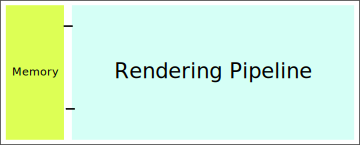
\includegraphics[width=12.5cm,keepaspectratio]{pics/pipeline/RenderingPipelineMemoryPipeline}
\end{frame}

\begin{frame}
\frametitle{Rendering Pipeline / Zobrazovací řetězec}
  \scriptsize
	\begin{itemize}
		\item Rendering Pipeline is divided into 2 parts: vector and raster.
    \item Splitting element is rasterization.
	\end{itemize}
	\begin{itemize}
		\item Zobrazovací řetěžec je rozdělen na 2 části - vektorovou a rastrovou.
    \item Dělícím prvkem je rasterizace.
	\end{itemize}
	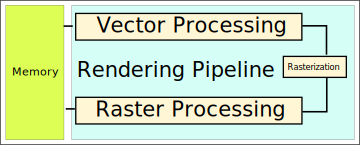
\includegraphics[width=12.5cm,keepaspectratio]{pics/pipeline/RenderingPipelineVectorRaster}
\end{frame}

\begin{frame}
\frametitle{Vector Part / Vektorová část}
  \scriptsize
	\begin{itemize}
		\item The main goal of vector part is to transform geometry.
    \item It processes vertices, primitives, it performs transformations, clipping, cullling, tessellation, projection,...
	\end{itemize}

	\begin{itemize}
		\item Hlavním úkolem vektorové části je transformace geometrie.
    \item Počítá vertex, primitiva, provádí transformace, ořez, teselaci, projekci, ...
	\end{itemize}

	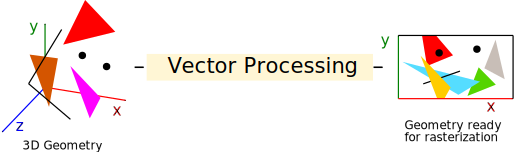
\includegraphics[width=12.5cm,keepaspectratio]{pics/pipeline/pipeline_vector_overview}
\end{frame}

\begin{frame}
\frametitle{Rasterization / Rasterizace}
  \scriptsize
	\begin{itemize}
    \item The goal of rasterization is to convert vector graphics elements (triangles, lines, points) to fragments.
	\end{itemize}

	\begin{itemize}
    \item Cílem rasterizace je převod vektorových grafických elementů (trojúhelníky, čáry, body) na fragmenty.
  \end{itemize}
	
\includegraphics[width=12.5cm,keepaspectratio]{pics/pipeline/rasterization_overview}
\end{frame}

\begin{frame}
\frametitle{Raster Part / Rastrová část}
  \scriptsize
	\begin{itemize}
		\item The main goal of raster part is to process fragments.
    \item It colors fragment, performs per fragment operations, depth test, stencil test, blending, ...
	\end{itemize}

	\begin{itemize}
		\item Hlavním úkolem rastrové části je výpočet fragmentů.
    \item Obarvuje fragment, provádí per fragment operace, hloubkový test, stencil test, blending, ...
	\end{itemize}
  
\includegraphics[width=12.5cm,keepaspectratio]{pics/pipeline/pfo_overview}
\end{frame}


\begin{frame}
\frametitle{Vector Part / Vektorová část}
  \scriptsize
	\begin{itemize}
		\item Vector Part is composed of many blocks.
    \item Some of the blocks are programable, some can be skipped.
	\end{itemize}
	\begin{itemize}
		\item Vektorová část řetězce je složena z mnoha bloků.
    \item Některé bloky jsou programovatelné a některé vynechatelné.
	\end{itemize}
	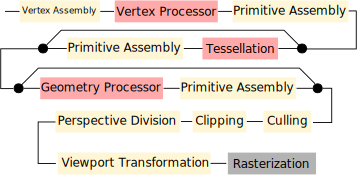
\includegraphics[width=12.5cm,keepaspectratio]{pics/pipeline/RenderingPipelineVector}
\end{frame}

\begin{frame}
\frametitle{Simplified vector part / Zlednodušená Vektorová část}
  \scriptsize
	\begin{itemize}
		\item If we remove optional blocks, the pipeline looks like this.
	\end{itemize}
	\begin{itemize}
		\item Pokud vynecháme volitelné bloky, zůstane zjednodušená vektorová část řetězce.
	\end{itemize}
	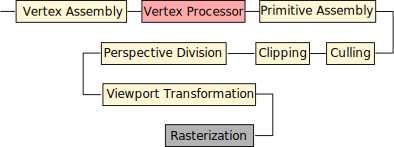
\includegraphics[width=12.5cm,keepaspectratio]{pics/pipeline/simplified_pipeline}
\end{frame}

\begin{frame}
\frametitle{Vertex Assembly, vertex processor, primitive assembly}
  \scriptsize
	\begin{itemize}
		\item Vertex Assembly creates vertices.
    \item Vertex processor transforms vertices.
    \item Primitive assembly creates base primitives from transformed vertices.
  \end{itemize}
	\begin{itemize}
		\item Vertex Assembly sestavuje vrcholy
    \item Vertex processor transformuje vrcholy
    \item Primitive assembly sestavuje základní primitiva.
	\end{itemize}
	
\includegraphics[width=12.5cm,keepaspectratio]{pics/pipeline/OpenGL460PipelineVertexShader}
\end{frame}

\begin{frame}
\frametitle{Vertex, Vertex Assembly}
  \scriptsize
	\begin{itemize}
		\item Vertex is a structure of vertex attributes.
    \item Vertex Assembly unit reads data from memory and forms vertices.
	\end{itemize}

	\begin{itemize}
		\item Vertex je struktura vertex atributů
    \item Vertex Assembly jednotka se stará o sestavování vrcholů z bufferů.
	\end{itemize}
	\begin{picture}(120,150)
		\put(0,0){\includegraphics[width=12.5cm,keepaspectratio]{pics/pipeline/vertex}}
	\end{picture}
	\begin{picture}(60,40)
		\put(50,0){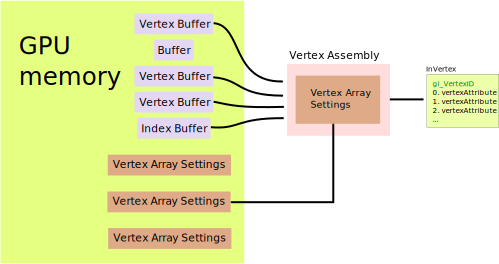
\includegraphics[width=8cm,keepaspectratio]{pics/pipeline/vertexAssembly}}
	\end{picture}
\end{frame}

\begin{frame}
\frametitle{Vertex Assembly / indexing}
  \scriptsize
	\begin{itemize}
		\item Vertex Assembly can utilize indexing
    \item Vertex Cache - already processed vertices do not have to be processed again
	\end{itemize}
	\begin{itemize}
		\item Vertex Assembly může využít indexování
    \item Vertex Cache - jednou propočítané vrcholy není třeba počítat znovu
	\end{itemize}
	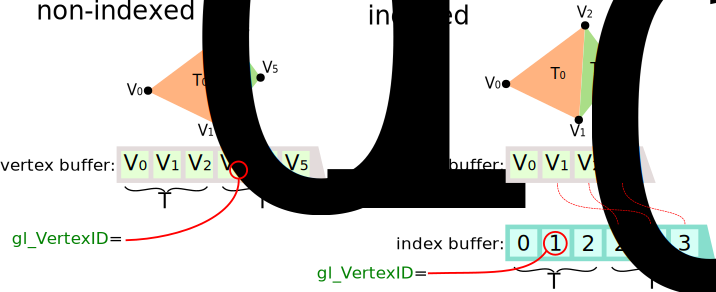
\includegraphics[width=12.5cm,keepaspectratio]{pics/pipeline/drawElements}
\end{frame}

\begin{frame}
\frametitle{Vertex Processor}
  \scriptsize
	\begin{itemize}
		\item Vertex Processor executes vertex shader.
    \item Vertex Shader is user program.
    \item The goal is to transform input vertex structure to output vertex structure.
	\end{itemize}

	\begin{itemize}
		\item Ve Vertex Processoru běží vertex shader.
    \item Vertex Shader je uživatelem specifikovaný program.
    \item Cílem je transformovat vstupní vrchol na výstupní vrchol.
	\end{itemize}
	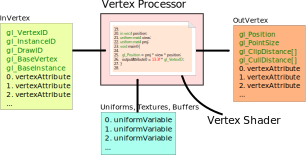
\includegraphics[width=10.5cm,keepaspectratio]{pics/pipeline/vertexShader}
\end{frame}

\begin{frame}
\frametitle{Primitive Assembly}
  \scriptsize
	\begin{itemize}
		\item Primitive Assembly unit creates base primitives.
    \item Output of the unit is one of the three base primitives (triangles, lines, points).
    \item The units is guided by the primitive type (Triangles, Triangle Strip, Triangle Fan, Line Strip, Adjacency, Patch, ...)
	\end{itemize}

	\begin{itemize}
		\item Primitive Assembly jednotka sestavuje primitiva.
    \item Cílem je podle nastavení sestavovat trojúhelníky, úsečky, vrcholy.
    \item Základní primitiva (trojúhleník, úsečka) mohou být součástí složitějších primitive.
    \item Triangle Strip, Triangle Fan, Line Strip, Triangle Adjacency, Patch, ...
	\end{itemize}
	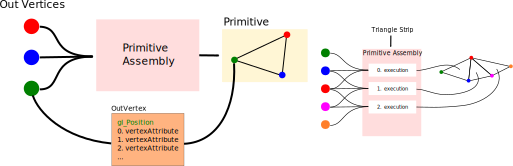
\includegraphics[width=12.5cm,keepaspectratio]{pics/pipeline/PrimitiveAssembly}
\end{frame}

\begin{frame}
\frametitle{Culling, clipping}
  \scriptsize
	\begin{itemize}
		\item Clipping, Culling, Perspective Divide and Viewport Transformation is performed between primitive assembly unit and rasterization.
    \item Culling discards back facing triangles.
    \item Clipping clips triangles that are not completely inside view-frustum.
    \item Perspective division shrinks objects that are further from the camera.
    \item Viewport Transformation transforms geometry to match screen resolution.
	\end{itemize}
	\begin{itemize}
    \item Mezi rasterizací a sestavením primitiv se provádí ořez, zahazování odvrácených trojúhelníků, perspektivní dělení a viewport transformace.
    \item Clipping ořezává primitiva, která jsou jen částečně v pohledovém jehlanu.
    \item Perspektivní dělení zmenšuje objekty, které jsou dál od kamery.
    \item Viewport transformace převádí objekty na rozměr obrazovky.
	\end{itemize}
	
\includegraphics[width=12.5cm,keepaspectratio]{pics/pipeline/OpenGL460PipelineClipping}
\end{frame}

\begin{frame}
\frametitle{Culling}
  \scriptsize
	\begin{itemize}
		\item Culling removes triangles that are backfacing or front facing the camera.
    \item The state of triangle orientation is decided by vertex winding.
    \item It is possible to discard backfacing or frontfacing triangles.
    \item Is is also possible to specify what is backfacing side (clock wise/counter clock wise vertices).
    \item Just for 2 manifold objects or scenes with restricted camera movement.
    \item Performance can be doubled with Culling.
	\end{itemize}
	\begin{itemize}
		\item Culling se stará o zahazování odvrácených trojúhelníků.
    \item Odvrácenost je rozhodnuta na základě pořadí vrcholů.
    \item Je možné nastavit, jestli je trojúhelník přivrácený nebo odvrácený, pokud jsou vrcholy po nebo proti směru hodinových ručiček.
    \item Výkon vykreslování může být zdvojnásoben díky Cullingu.
	\end{itemize}
	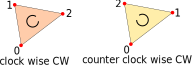
\includegraphics[width=8.5cm,keepaspectratio]{pics/pipeline/culling}
\end{frame}

\begin{frame}
\frametitle{Clipping, near-plane clipping}
  \scriptsize
	\begin{itemize}
		\item If a primitive is only partially inside view-frutum, it needs to be clipped.
    \item Only near-plane clipping is necessary.
    \item If the result is quadrangle, it can be replaced with two sub-triangles.
	\end{itemize}
	\begin{itemize}
		\item Pokud je primitivum jen částečně uvnitř pohledového jehlanu, je potřeba jej oříznout.
    \item Obvykle stačí oříznout pomocí blízké ořezové roviny (near-plane).
    \item Pokud vznikne čtyřúhelník, je možné jej nahradit dvěma trojúhelníky.
	\end{itemize}
	\begin{picture}(120,150)
		\put(0,0){\includegraphics[width=4.5cm,keepaspectratio]{pics/pipeline/clip}}
	\end{picture}
	\begin{picture}(60,40)
		\put(25,0){\includegraphics[width=4cm,keepaspectratio]{pics/pipeline/clip_variants}}
	\end{picture}
\end{frame}

\begin{frame}
\frametitle{Perspective Divide / Perspektivní dělení}
  \scriptsize
	\begin{itemize}
		\item Perspective Division unit converts hommogeneous coordinates to cartesian coordinates.
    \item It divides $x,y,z$ using $w$. The $w$ contains distance from camera.
    \item After division, $x,y,z \in [-1,+1]$ which is called normalized device coordinates (NDC).
    \item Division is expensive operation, specialized HW performs it fasters.
	\end{itemize}
	\begin{itemize}
		\item Blok perspektivního dělení převádí homogenní souřadnice na kartézské.
    \item Dělí se pomocí W, ve kterém je uložena hloubka. Tím se zmenšují objekty, které jsou dál od kamera.
    \item Po perspekvitním dělení všechny vrcholy leží v rozsahu $[-1,+1]$ - normalized device coordinates.
    \item Dělení je drahá operace, specializovaný HW ji provede rychleji.
	\end{itemize}
	\includegraphics[width=6.5cm,keepaspectratio]{pics/pipeline/PerspectiveDivision}
\end{frame}

\begin{frame}
\frametitle{Viewport Transform / Viewport transformace}
  \scriptsize
	\begin{itemize}
		\item Viewport transformation converts NDC to screen resolution.
	\end{itemize}
	\begin{itemize}
		\item Blok viewport transformace transformuje normalizované souřadnice na rozlišení plátna.
	\end{itemize}
	\includegraphics[width=8.5cm,keepaspectratio]{pics/pipeline/ViewportTransformation}
\end{frame}

\begin{frame}
\frametitle{Tessellation / Teselace}
  \scriptsize
	\begin{itemize}
		\item Tessellation is composed of 2 programable parts and hardware primitive generator.
    \item The goal of tessellation is to add geometric details.
	\end{itemize}
	\begin{itemize}
		\item Tesselace je složena zde 2 programovatelných processorů a hardwarového generátoru primitiv.
    \item Cíl teselace je přidání geometrických detailů.
	\end{itemize}
	
\includegraphics[width=12.5cm,keepaspectratio]{pics/pipeline/OpenGL460PipelineTessellationShaders}
\end{frame}

\begin{frame}
\frametitle{Geometry processor, transform feedback}
  \scriptsize
	\begin{itemize}
		\item Geometry processor inputs and outputs are primitives.
    \item The goal is to change, generate primitives.
    \item The stream of primitives can be sent to buffer.
	\end{itemize}
	\begin{itemize}
		\item Geometry processor transformuje primitiva.
    \item Transform feedback může primitiva přeposlat zpět do bufferu.
	\end{itemize}
	
\includegraphics[width=12.5cm,keepaspectratio]{pics/pipeline/OpenGL460PipelineGeometryShader}
\end{frame}

\begin{frame}
\frametitle{Rasterization / Rasterizace}
  \scriptsize
	\begin{itemize}
		\item Rasterization produces fragments.
    \item Fragment is date structure that is created in the location of sampling point.
    \item Sampling point is usualy in the center of pixel.
    \item The situation is more complicated with the use of multisampling.
    \item If a sampling point is located inside a triangle, a fragment is created for corresponding pixel.
	\end{itemize}
	\begin{itemize}
		\item Rasterizace produkuje fragmenty.
    \item Fragment je datová struktura, která vznikne na pozici vzorku (sampling point).
    \item Vzorkovací bod je obvykle uprostřed pixelu.
    \item Situace je komplikovanější při využití multi-samplingu.
    \item Pokud leží vzorkovací bod uvnitř trojúhelníku, vznikne fragment pro daný pixel.
	\end{itemize}
	\begin{figure}[h]
		\includegraphics[width=10cm,keepaspectratio]{pics/pipeline/rasterization.pdf}
	\end{figure}
\end{frame}

\begin{frame}
\frametitle{Rasterization and Interpolation / Rasterizace a interpolace}
  \scriptsize
	\begin{itemize}
		\item Out Vertices are composed of n vertex attributes.
    \item Rasterization produces fragments -- data structure -- which is composed of fragment attributes with the same user specific fragment attributes.
    \item Barycentric interpolation is used to transform three vertex data structures to many fragment data structures.
	\end{itemize}
	\begin{itemize}
		\item Vertexy jsou před rasterizací popsány pomocí n-tice atributů
    \item Rasterizace produkuje fragmenty, pokud jejich střed leží uvnitř primitiva
    \item Po rasterizaci jsou tyto atributy vloženy do fragmetů pomocí interpolace
	\end{itemize}
	\begin{figure}[h]
		\includegraphics[width=10cm,keepaspectratio]{pics/pipeline/interpolation.pdf}
	\end{figure}
\end{frame}

\begin{frame}
\frametitle{Barycetric coordinates / Barycentrické koordináty}
	\begin{figure}[h]
		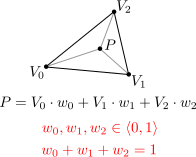
\includegraphics[width=8cm,keepaspectratio]{pics/pipeline/barycentrickekoordinaty.pdf}
	\end{figure}
\end{frame}

\begin{frame}
\frametitle{2D Barycentric coordinates / Barycentrické koordináty ve 2D}
  \scriptsize
	\begin{itemize}
		\item 2D barycentrics are computed as ratio between the area of the triangle and the areas of its sub-triangles. 
	\end{itemize}
	\begin{itemize}
		\item Barycentrické koordináty ve 2D jsou spočítaný jako poměr obsahů.
	\end{itemize}
	\begin{figure}[h]
		\includegraphics[width=8cm,keepaspectratio]{pics/pipeline/barycentric2D.pdf}
	\end{figure}
\end{frame}

\begin{frame}
\frametitle{Perspective distortion / Perspektivní zkreslení}
  \scriptsize
	\begin{itemize}
		\item Vertex attributes can be interpolated in the projection plane or in the 3D space.
    \item Interpolation in the 3D space is correct.
    \item In order to convert 2D interpolation to 3D interpolation, the perspective correction is required (OpenGL supports this natively / can be turned off)
	\end{itemize}
	\begin{itemize}
		\item Vertex atributy se mohou interpolovat v rovině průmětny nebo v prostoru scény
    \item Aby se mohlo interpolovat v prostoru scény, musí se provést perspektivní korekce
      (v OpenGL automaticky/lze vypnout)
	\end{itemize}
	\begin{figure}[h]
		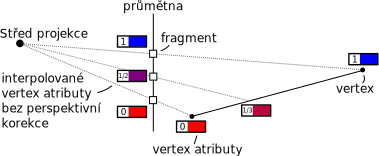
\includegraphics[width=10cm,keepaspectratio]{pics/pipeline/prespektivni_korekce.pdf}
	\end{figure}
\end{frame}

\begin{frame}
\frametitle{Fragment Processor}
  \scriptsize
	\begin{itemize}
		\item Fragment shader is executed inside fragment processor.
    \item Fragment Shader is user program.
    \item The goal of the shader is to transform input fragment to output fragments.
    \item Multiple Render Target - support for rendering into multiple 2D arrays (renderbuffers / textures).
	\end{itemize}
	\begin{itemize}
		\item Ve Fragment Processoru běží fragment shader.
    \item Fragment Shader je uživatelem specifikovaný program.
    \item Cílem je transformovat vstupní fragment na výstupní fragment.
    \item Multiple Render Target.
	\end{itemize}
	\begin{figure}[h]
		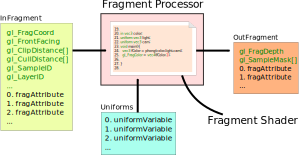
\includegraphics[width=8cm,keepaspectratio]{pics/pipeline/FragmentShader.pdf}
	\end{figure}
\end{frame}

\begin{frame}
\frametitle{Early fragment tests / Brzké testy a operace}
	\begin{figure}[h]
	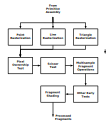
\includegraphics[width=7cm,keepaspectratio]{pics/pipeline/OpenGL460PipelineRaster}
	\end{figure}
\end{frame}

\begin{frame}
\frametitle{Late fragment tests and operations}
	\begin{figure}[h]
	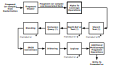
\includegraphics[width=12.5cm,keepaspectratio]{pics/pipeline/OpenGL460PipelineFragmentShader}
	\end{figure}
\end{frame}

\begin{frame}
\frametitle{PFO - depth test}
	\begin{figure}[h]
	\includegraphics[width=10.5cm,keepaspectratio]{pics/pipeline/PFO}
	\end{figure}
\end{frame}


\begin{frame}
\frametitle{OpenGL 4.6 pipeline}
  \begin{figure}[h]
  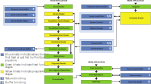
\includegraphics[width=10cm,keepaspectratio]{pics/pipeline/OpenGL460Pipeline}
  \end{figure}
\end{frame}


